\section{Ideal Rigid Body (IRB) Bound}

\begin{frame}{Ideal Rigid Body (IRB) Bound}
\begin{itemize}
    \item Post-hoc model which selects an impulse pair (Normal and Tangential Impulses) from the impulse space
    \item Impulse space is defined by energy allowable impulses given pre-impact energy (no increases in energy due to impact)
    \item Impulse pair is chosen to minimize $\ell_2$ norm of post-impact velocity
\end{itemize}     
     \begin{figure}
        \centering
        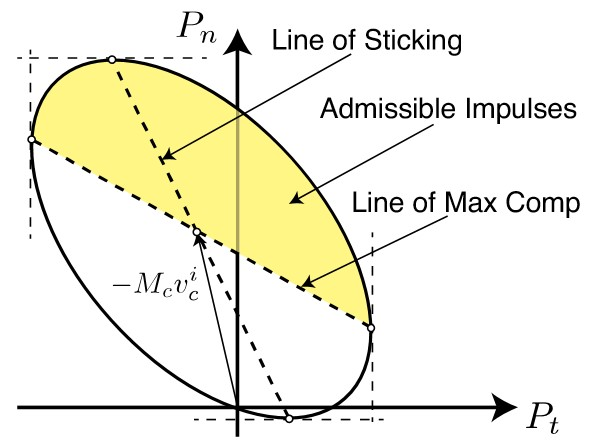
\includegraphics[scale=0.6]{figures/energyEllipse.jpg}
        \caption{Energy Ellipse\cite{nima2}}
        \label{fig:energyEllipse}
\end{figure}

\end{frame}

\subsection{Implementing the IRB Bound}
\begin{frame}{Implementing the IRB Bound}
    \begin{itemize}
        \item Initial energy, KE $= \frac{1}{2}v_{pre}^T*\textbf{M}*v_{pre}$
        \item Post-impact velocity, $v_{predicted} = v_{pre} + \textbf{M}^{-1} \textbf{J}^T \textbf{P}^T$
            \begin{itemize}
                \item $\textbf{M}$ -- generalized mass matrix
                \item $\textbf{J}$ -- contact Jacobian
                \item $\textbf{P}$ -- impulse vector
            \end{itemize}
        \item Run \textit{fmincon} to find the best pair of impulses using normalized error as cost with the energy ellipse as a primary constraint
        \item Even though this is a flexible post-hoc model, we were seeing large errors from the IRB predicted impulses (similar to Nima's paper)
        
    \end{itemize}    
\end{frame}

%surprisingly high error from normal IRB

%IRB with width/Torque
% found that width could be as high as roughly 20 mm, which is highly      unlikely given the actual dimensions of the ellipse and the material properties.

%angle correlations/other correlations
\subsection{IRB with Torque}
\begin{frame}{IRB with Torque}
One idea Prof. Posa suggested to explain the errors we were seeing (discussed further in a later section) is to remove the single point contact assumption and treat the impact as if it occurs over a region.
    \begin{figure}
        \centering
        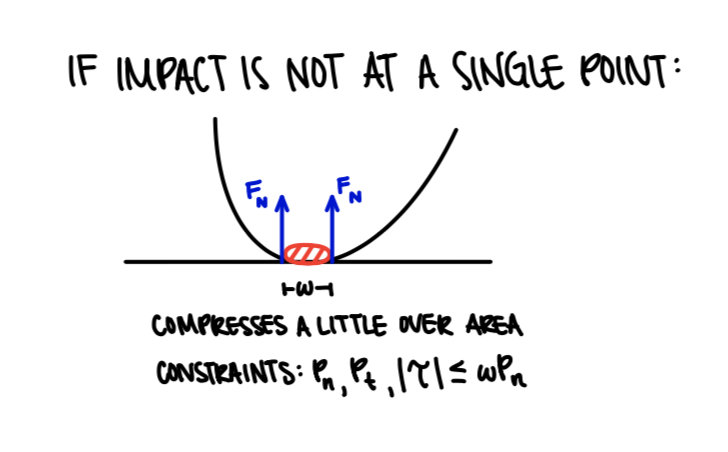
\includegraphics[scale=0.6]{figures/IRBTorque.png}
        \caption{IRB Torque Diagram}
        \label{fig:IRBTorque}
\end{figure}
\end{frame}

\begin{frame}{IRB with Torque}
\begin{itemize}
    \item Adds an additional torque ($|\tau| = w_{patch}*\textbf{P}_n$)
    \item Additional constraint ($|w_{patch}|\leq w_{max}$)
    \item The calculation is still $v_{predicted} = v_{pre} + \textbf{M}^{-1} \textbf{J}^T \textbf{P}^T$ however \textbf{J} and \textbf{P} now have a third row: 
\end{itemize}



\centering
\[
    \textbf{J} =
        \left [
        \begin{array}{ccc}
             & \textbf{d} & \\
             & \textbf{n} & \\
             0 & 0 & 1 \\
        \end{array}
        \right ],\
            \textbf{P} = 
       \left [
        \begin{array}{c}
            \textbf{P}_n \\
            \textbf{P}_t \\
            \tau   \\
        \end{array}
        \right ]
\]

\begin{itemize}
    \item This additional decision variable ($\tau$) should reduce error and lead to more accurate predictions from the IRB Bound

\end{itemize}   

  
\end{frame}
    
\begin{frame}{IRB with Torque's Effect on Error}
    \begin{figure}
        \centering
        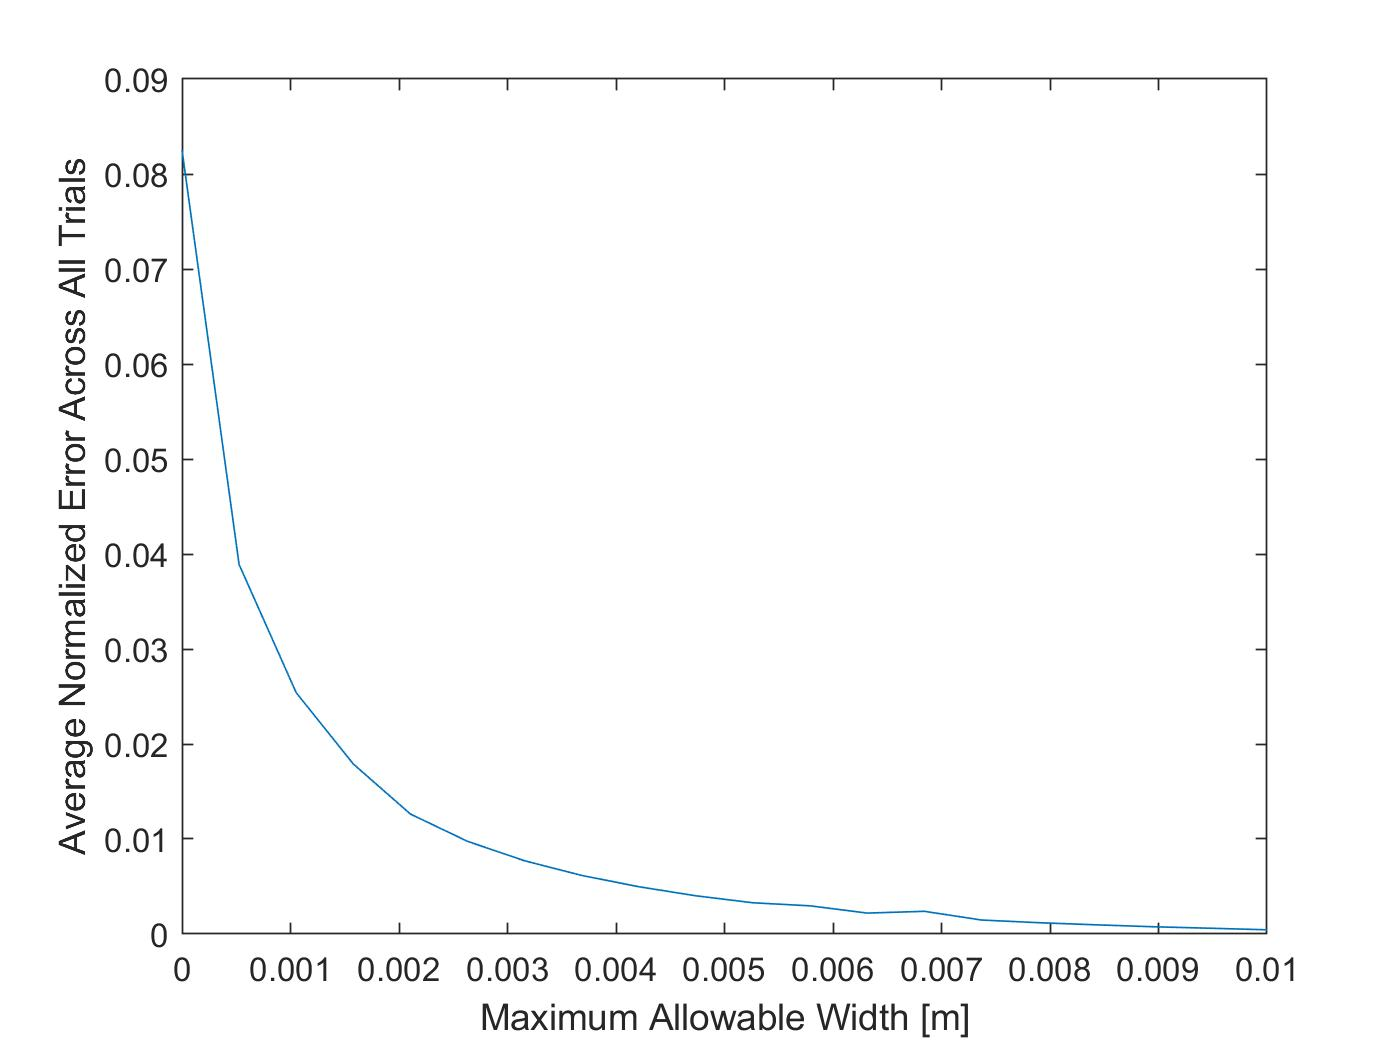
\includegraphics[scale=0.15]{figures/IRBErrorVsMaxWidth.jpg}
        \caption{Average Error Across 1000 Random Trials Vs. Maximum Allowable Width}
        \label{fig:IRBErrorVSMaxWidth}
    \end{figure}
\end{frame}

%TAKEAWAYS FROM PLOT ^^^^^
%Small Patch size has significant effect in lowering error (1mm cuts average error in half)
%Patch size isn't a sole solution however, since to get really low errors, you need unrealistically large widths
%As a good sanity check however, as the max width increases and becomes nearly unconstrained, the error approaches 0

\begin{frame}{IRB Trends}
One of the things we did to try to understand how the IRB Bound worked was plotting different properties against each other. 

%\begin{figure}
    %\centering
    %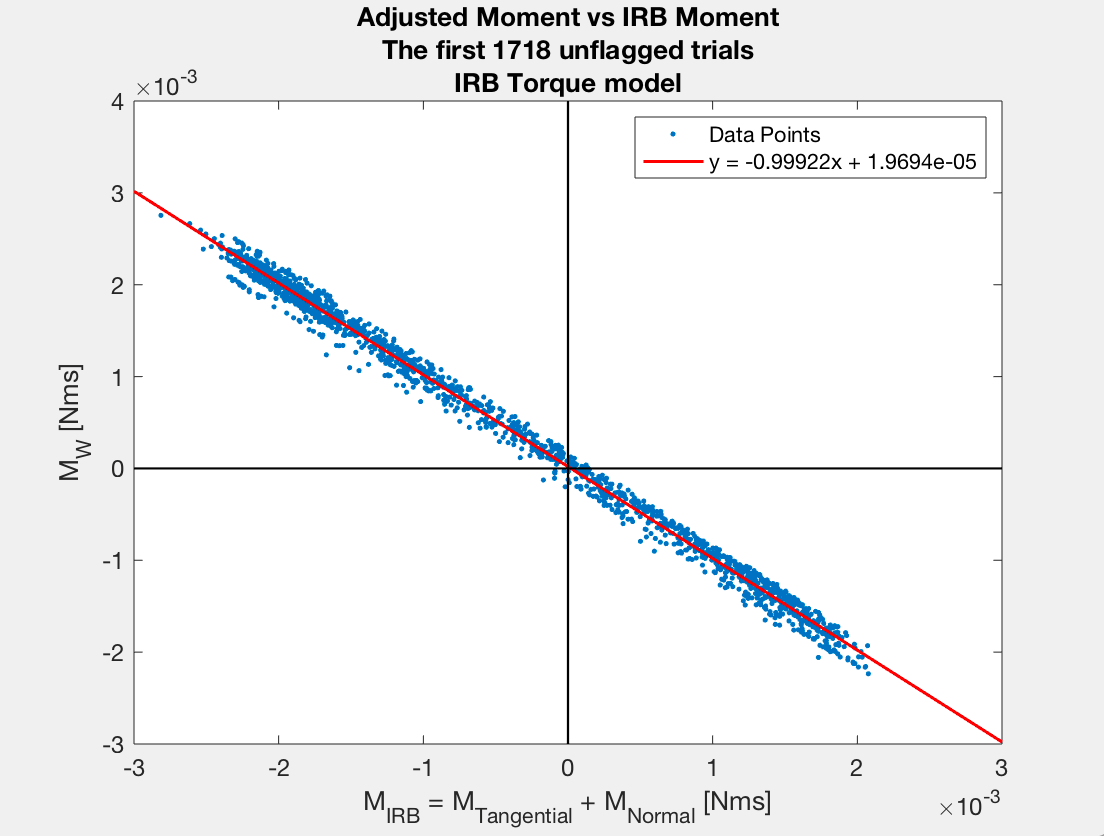
\includegraphics[scale=0.18]{figures/Trends.png}
    %\caption{Torque against IRB moment}
    %\label{fig:MomentsError}
%\end{figure}

\begin{figure}
    \centering
    \begin{minipage}{.5\textwidth}
      \centering
      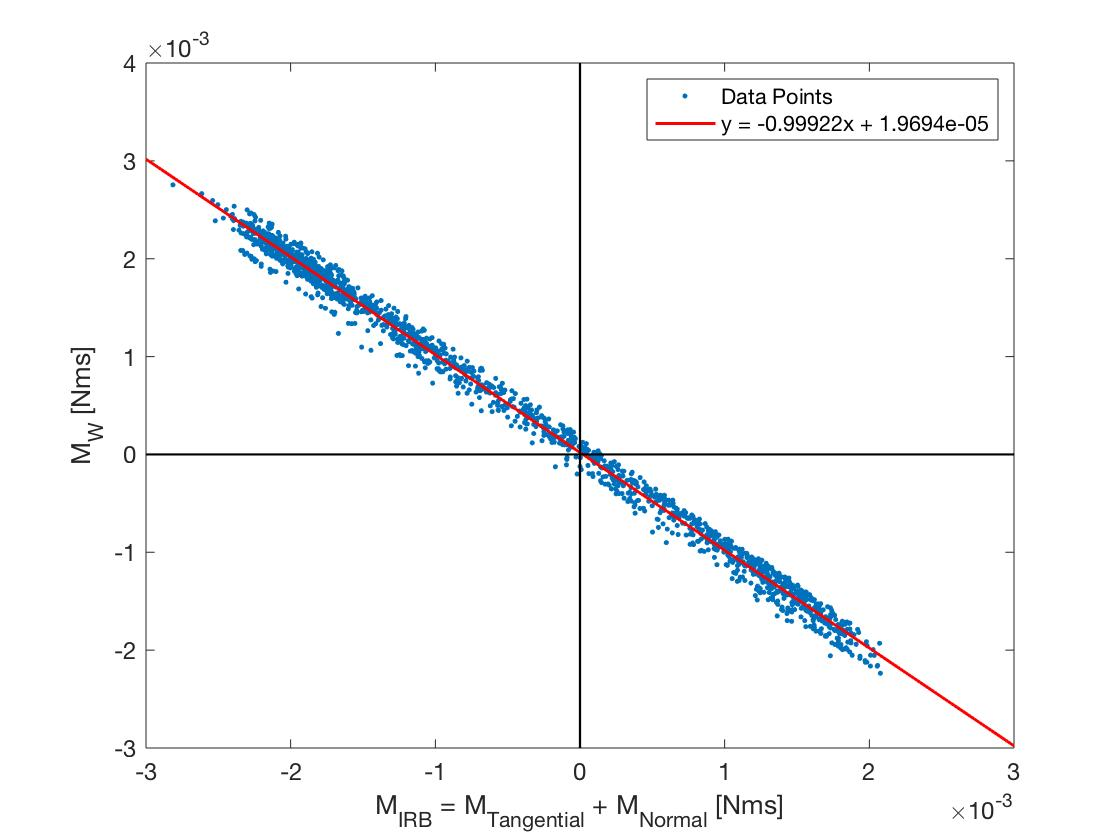
\includegraphics[width=1\linewidth]{figures/MomentProp2.jpg}
    \captionof{figure}{IRB Moment vs Torque}
      \label{fig:contourWM2}
    \end{minipage}%
    \begin{minipage}{.5\textwidth}
      \centering
      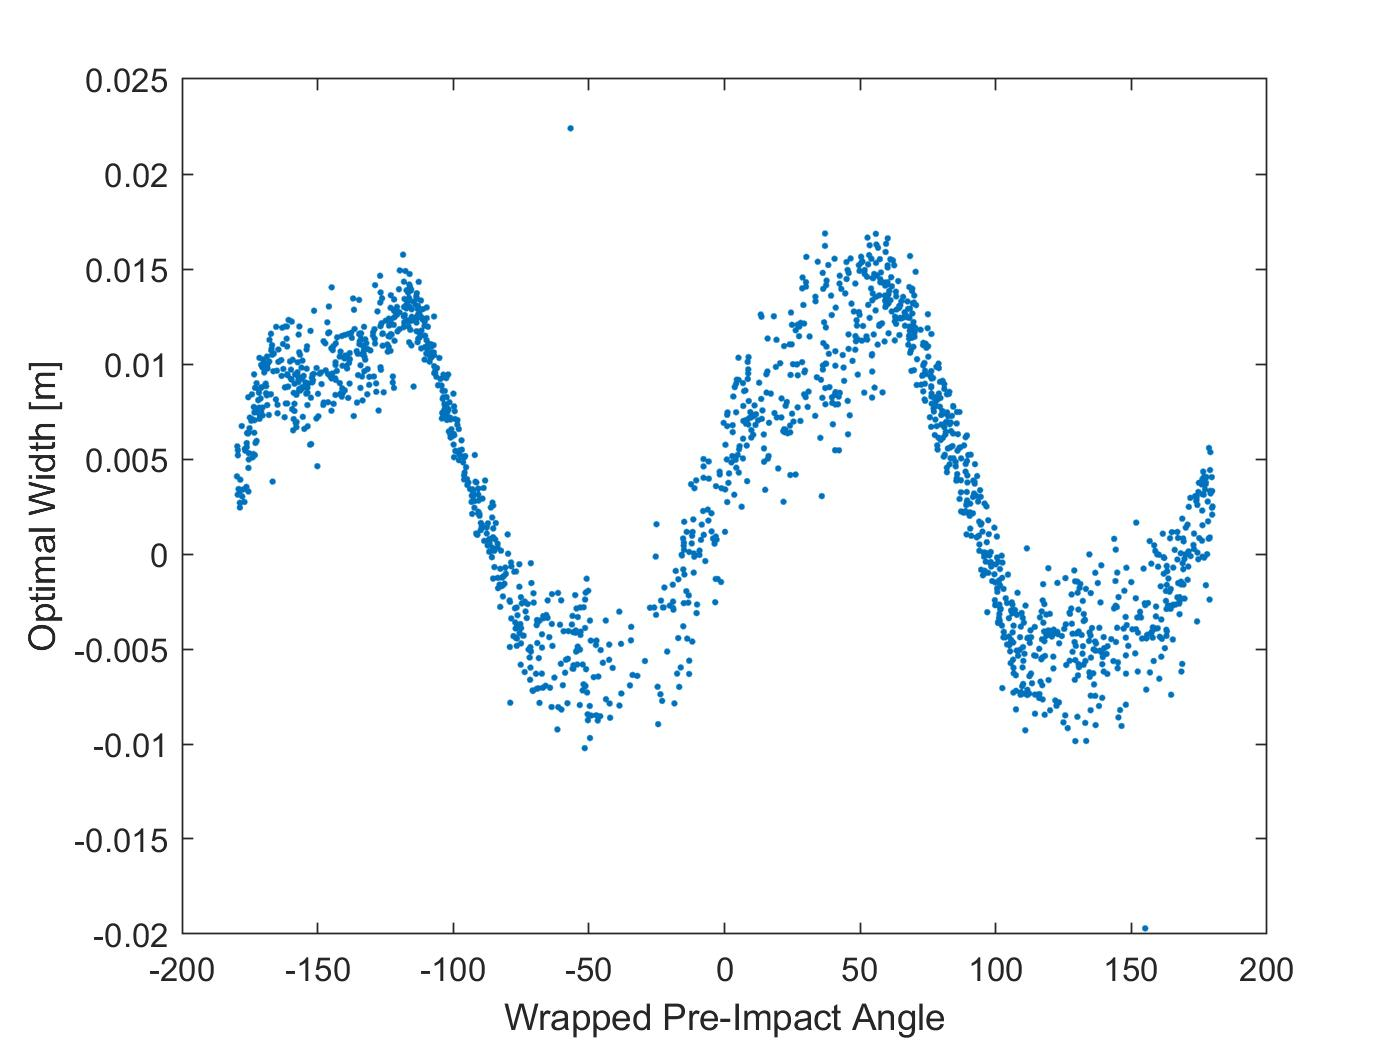
\includegraphics[width=1\linewidth]{figures/ellipseAngleWidth.jpg}
    \captionof{figure}{Optimal Width vs Angle}
      \label{fig:histWM2}
    \end{minipage}
\end{figure}    
    
\end{frame}